% Use only LaTeX2e, calling the article.cls class and 12-point type.

\documentclass[12pt]{article}

% Users of the {thebibliography} environment or BibTeX should use the
% scicite.sty package, downloadable from *Science* at
% www.sciencemag.org/about/authors/prep/TeX_help/ .
% This package should properly format in-text
% reference calls and reference-list numbers.

\usepackage{verbatim}

% Allows for multiple line comments using \begin{comment} and \end{comment}

\usepackage{amsmath}
%\renewcommand{\vec}[1]{\mathbf{#1}}

\usepackage{hyperref}

\usepackage{graphicx}

\usepackage{float}
\usepackage{caption}
\usepackage{subcaption}

% Use times if you have the font installed; otherwise, comment out the
% following line.

\usepackage{times}

% The preamble here sets up a lot of new/revised commands and
% environments.  It's annoying, but please do *not* try to strip these
% out into a separate .sty file (which could lead to the loss of some
% information when we convert the file to other formats).  Instead, keep
% them in the preamble of your main LaTeX source file.


% The following parameters seem to provide a reasonable page setup.

\topmargin 0.0cm
\oddsidemargin 0.2cm
\textwidth 16cm 
\textheight 21cm
\footskip 1.0cm


%The next command sets up an environment for the abstract to your paper.

\newenvironment{sciabstract}{%
\begin{quote} \bf}
{\end{quote}}


% If your reference list includes text notes as well as references,
% include the following line; otherwise, comment it out.

\renewcommand\refname{References and Notes}

% The following lines set up an environment for the last note in the
% reference list, which commonly includes acknowledgments of funding,
% help, etc.  It's intended for users of BibTeX or the {thebibliography}
% environment.  Users who are hand-coding their references at the end
% using a list environment such as {enumerate} can simply add another
% item at the end, and it will be numbered automatically.

\newcounter{lastnote}
\newenvironment{scilastnote}{%
\setcounter{lastnote}{\value{enumiv}}%
\addtocounter{lastnote}{+1}%
\begin{list}%
{\arabic{lastnote}.}
{\setlength{\leftmargin}{.22in}}
{\setlength{\labelsep}{.5em}}}
{\end{list}}


% Include your paper's title here

\title{Projecting domestic species invasion spread using commodity flow pathways} 


% Place the author information here.  Please hand-code the contact
% information and notecalls; do *not* use \footnote commands.  Let the
% author contact information appear immediately below the author names
% as shown.  We would also prefer that you don't change the type-size
% settings shown here.

\author
% {Nathan Wikle,$^{1\ast}$ Ryan Yan,$^{2}$ Ashish Gauli$^{3}$\\
{Ashish Gauli,$^{1,2}$ Nathan Wikle,$^{1,3}$ Ryan Yan,$^{1,4}$\\ 
Dr. Louis Gross,$^{1,5}$ Dr. Daniel Simberloff,$^{5}$ Angela Chuang,$^{5}$ Cedric Landerer$^{5}$\\
\\
\normalsize{$^{1}$National Institute for Mathematical and Biological Synthesis (NIMBioS)}\\
% \normalsize{spot for address}\\
\normalsize{$^{2}$Biology and Computer Science, Fisk University}\\
% \normalsize{spot for address}\\
\normalsize{$^{3}$Mathematics, Truman State University}\\
% \normalsize{spot for address}\\
\normalsize{$^{4}$Mathematical Biology, College of William and Mary}\\
% \normalsize{spot for address}\\
\normalsize{$^{5}$Ecology and Evolutionary Biology, University of Tennessee}\\
% \normalsize{spot for address}\\
\\
% email for correspondence
% \normalsize{$^\ast$To whom correspondence should be addressed; E-mail:  jsmith@wherever.edu.}
}

% Include the date command, but leave its argument blank.

\date{\today}



%%%%%%%%%%%%%%%%% END OF PREAMBLE %%%%%%%%%%%%%%%%



\begin{document} 

% Double-space the manuscript.

\baselineskip24pt

% Make the title.

\maketitle 


 \begin{sciabstract}
Abstract: Models to create projections of invasive species spread are critical in identifying high priority shipping centers and pathways of bioinvasion, essential information in the prevention of environmental and economic harm caused by invasive species.  Research into the development of large-scale models of biological invasion have largely been targeted towards network models of international shipping pathways. However, the majority of models for domestic invasions have been confined to basic diffusive spread. Nevertheless, many species of harmful pests are known to travel long-distances through the shipment of specific commodities.  For example, \textit{Solenopsis invicta}, the red imported fire ant, can travel via turf shipments within the United States. The availability of commodity flow data suggests that a model utilizing domestic freight as the dominant vector of dispersal may be a promising yet unexplored avenue of research in invasive species ecology. To this end, we utilize data on domestic commodity flows from the Freight Analysis Framework to create projections of invasive species spread. Furthermore, we introduce the Commodity Flow Visualization System, a tool designed to aid in the visualization of commodity shipments within the United States.
\end{sciabstract}



\section*{Introduction}

Modern societies are increasingly dependent upon a complex network of global and national trade which facilitates the quick transport of all types of goods.  Although this interconnectedness has led to the flourishing of today's global economy, the increased volume of trade has had serious consequences for ecological health worldwide.  In particular, human commerce is the foremost vector for the global dissemination of invasive species, which has resulted in large-scale ecosystem destruction and immense economic costs to invaded regions (Mack et al. 2000).  Understanding the role of commodity movement in the spread and introduction of invasive species is a crucial step in their prevention and control.  In the long term, we aim to provide governments with the information to most effectively halt the spread of invading species at their most likely source.

Due to its prevalence and outsized role as a conduit for invasive species, the global maritime shipping network has been thoroughly analyzed to identify common hotspot ports and pathways of invasion.  Maritime shipping alone accounts for over 90 percent of the world's trade (Kaluza et al. 2009), and careful consideration has been taken to characterize its role in the spread of foreign species.  Data from the Automated Identification System (AIS) technology, a real-time tracking system installed on most large ships, has allowed the construction and analysis of the global shipping network by Kaluza et al. (2009).  This network's characterization as a small-world and scale-free network suggests that it is particularly prone to the rapid dispersal of invasive species along its edges (Pastor-Satorras and Vespignani 2001).  Indeed, ballast water discharge and hull fouling of freight vessels are directly responsible for the transfer of many marine organisms (Ruiz et al. 2000).  And yet, transported species are not limited to marine species. Nonindigenous plant pest species have also been found regularly in cargo entering the United States (McCullough et al. 2006, Work et al. 2005), and even more species enter undetected (Work et al. 2005).

As a result, shipping pathway risk assessments are needed for efficient prevention and management of foreign species invasions (Hulme 2009).  Research in this area has largely been devoted to studying the global shipping network.  For example, Drake and Lodge applied a gravity model to identify probable pathways of marine invasion and identified specific hotspot ports most likely to distribute invasive species (2004).   Similarly, Seebens et al. identified hotspots of bioinvasion using maritime shipping data, and extended their model to consider port environmental conditions and biogeography when identifying probable pathways (2013).  In another study, Paini and Yemshanov used a Markov chain model to identify the most probable countries of origin for the invasion of the Khapra beetle invasion to Australian ports (2012).  Increasingly, network models have been used to investigate international species transport, however, the expansion of these networks to domestic modes of transportation has been limited (Hulme 2009).

The role of domestic freight shipping as a method of invasive species dispersal has been largely confined to an analysis of the domestic movement of imports entering the United States and Canada (Colunga-Garcia et al. 2009, Koch et al. 2010, Yemshanov et al. 2012).  Using domestic shipping data in conjunction with import data, the risk of foreign invasion to urban forest areas was assessed for specific regions in the United States.  Establishment rates were found to be low overall, except in a small subset of urban areas with high population density and a high volume of imports (Colunga-Garcia et al. 2009, Koch et al. 2010).  Similar analysis of Canadian imports reveals that establishment rates are lower, on average, than those found in the United States (Yemshanov et al. 2012).  Although key points of entry and invasion pathways were established for exotic pests, in all cases, the focus of these studies was on the establishment of new foreign species via imports; the dispersal of already established invasive species across the United States was never discussed.  

Research into domestic freight as a mode of species dispersal seems promising for multiple reasons.  First, there exists a substantial database on domestic commodity shipping within the United States.  Based largely on data collected by the U.S. Census Bureau in their Commodity Flow Survey (CFS), the Freight Analysis Framework (FAF) database contains aggregated data on freight shipments in the United States, separated by commodity type and mode of transportation (see \textit{Data Source} for more information).  The data are regularly used by state and regional departments of transportation in the creation of freight forecasting models (NCHRP Report 606 2008, Chow et al. 2010, Sivakumar and Bhat 2002), however, their potential value in bioinvasion literature remains untapped.  Second, it is widely believed that specific species are transported through domestic commodity shipments. For example, the USDA holds strict regulations on the shipment of soil from metropolitan areas known to house the Red Imported Fire Ant (USDA Fire Ant Program Manual 2010).  Thus, a network model of commodity flow in the United States could be utilized in identifying hotspots and pathways of bioinvasion. 

This idea has motivated our work this summer, and has led to the development of the following goals:

\begin{enumerate}

\item Develop a tool to visualize the flow of commodities within the United States using data obtained from the Federal Highway Administration.

\item Create projections of domestic invasive species spread using a stochastic model where dispersal occurs through a commodity freight network.

\item Use the aforementioned model to perform risk analyses to better inform managers challenged with controlling invasive species spread.

\end{enumerate}


\section*{Methodology}

\subsection*{Freight Data}


Shipping data were obtained from the Freight Analysis Framework (FAF), a database that combines data sources to create a complex freight movement summary of terrestrial commodity shipments between geographic regions within the United States. In particular, flow matrices have been created for 1997, 2002, 2007, and 2012, with additional flow forecasts from 2015 to 2040.  The 2007 and 2012 data contain 123 domestic regions, 74 of which are metropolitan areas, 33 the remainders of particular states, and 16 entire states, where no FAF metropolitan regions exist.  There are 43 commodity classes, as classified by the Standard Classification of Transported Goods (SCTG).  We retrieved FAF data for the following years: 1997, 2002, 2007, and 2012. Each line of data records an origin and destination, a particular commodity, mode of transportation, value of goods shipped, weight in kilotons, as well as metrics involving distance traveled. An extensive review of FAF methodology can be found in [FAF3].

%\paragraph*{Preliminary Network Analysis}

An effort was made to classify the large-scale domestic commodity shipping networks obtained from the FAF database.  Basic network topological features have been used to characterize many existing real-world networks, including the internet, the World Wide Web, biological networks (intracellular biochemical pathways, genetic regulatory networks, etc.), and a variety of transportation networks (Barrat et al. 2008).  These complex networks are often classified as having small-world and scale-free properties, an indication of the presence of important high-degree nodes known as hubs.  In particular, the worldwide air-transportation network (WAN) has been found to have heavy-tailed, power-law degree and strength distributions (Barrat et al. 2004, Guimera and Amaral 2004), while the global cargo-ship network (GCSN) has a right-skewed degree distribution, and power-law weight and strength distributions (Kaluza et al. 2009).  Because the WAN and GCSN are large-scale transportation networks, it was expected that the domestic shipping networks obtained from the FAF would have similar network characteristics - in particular, that the FAF networks would have small-world and scale-free properties.

However, an initial analysis of the FAF networks reveals a less structured topology.  As an example, consider the network of agricultural products transported by truck between the 123 FAF designated metropolitan regions of the United States.  A small-world network has the property that any two vertices can be traveled between by passing through a small number of intermediate vertices, while also requiring the existence of highly-clustered nodes.  This property can be measured by examining the relationship between the average shortest path length $\big \langle l \big \rangle$ and $M(l)$, the average number of nodes within a distance less than or equal to $l$ from any given vertex.  $M(l)$ is expected to increase exponentially in a small-world network (Barrat et al. 2008).  As shown in Figure~\ref{fig:plot length}, any two nodes in the agricultural commodity network can be reached within two steps.  However, because nodes in this network are highly connected ($\big \langle k \big \rangle = 80$), it is unclear if the observed relationship is a result of node clustering.  

The classification of the agricultural commodity network as scale-free is also ambiguous.  The degree distribution $P(k)$ for the network is shown in Figure~\ref{fig:degree dist}.  Notice that there is an increase in $P(k)$ as $k$ increases, and the network shows no evidence of a heavy-tail degree distribution.  However, when strength and edge weight distributions are considered, we observe that each is heavy-tailed and approximates a power-law distribution (Figure~\ref{fig:strength dist} and Figure~\ref{fig:weight dist}).  Thus, there appears to be a correlation between the weighted properties of the network and the network topologies.  Although these results are specific to the agricultural commodity network, they are largely representative of the many commodity flow networks found in the FAF database.  We believe that the difference in the degree and weighted property distributions is a characteristic of the highly aggregated node structure of the network, the spatial properties of the existing domestic infrastructure, and the addition of noise and variation into the data itself. A more thorough exploration of the statistical and topological properties is needed to correctly classify the shipping networks.

\subsection*{A Domestic Shipping Pathway Model}

Using a stochastic matrix model framework, we developed a methodology to project domestic invasive species spread using commodity pathways.  For this model, two important assumptions were made.  First, the invasive species of interest must be transported via a particular commodity or set of commodities and a specific mode of transportation.  Second, an initial domestic region has already been invaded by the species, and additional invasion can only occur domestically.  This means that additional establishment from foreign imports is no longer considered in the propagation of the species.  Thus, the model is restricted to domestic spread. However, it could potentially be coupled with a global model if desired.

Because the FAF data was regionally aggregated to  individual U.S. states in 1997 and 2002, our model considered the spread of a hypothetical invasive species within 51 geographic areas: the fifty states and Washington D.C.  If higher resolution data is available, this can be easily extended to $m$ regions.  A state vector $s_t$ represents the percentage of establishment of the species within each region in year $t$.  More specifically, $s_{t_i}$ is the percentage of establishment of region $i$ in year $t$, for $i = 1,2,..., m$.  Thus, at time $t=0$, the invaded regions should be initialized to 1, and all uninvaded regions to 0.    

In a given year $t$, it is assumed that the invading population will continue to grow in each region $i$ until the species has become fully established.  Thus, a logistic growth function $g$ is applied element-wise to $s_t$.  This is defined as
\[ 
	g(s_{t_i}) = \frac{s_{t_i} e^r}{1+s_{t_i} (e^r-1)}
\]
where $i=1,2,...,m$ and $r$ is the annual growth rate.  We have arbitrarily chosen $r$ to be 0.01, however, it is recommended that an estimated growth rate be used for the species in question.

Next, a transition matrix $P_t$ is created for year $t$ from the FAF data.  Each element $p_{t_{ij}}$ represents the proportion of a given commodity produced in state $j$ that is being exported to state $i$.  More specifically, 
\[
p_{t_{ij}} = \frac{w_{t_{ij}}}{\sum_{i=1}^{m} w_{t_{ij}}},  
\]
where $w_{t_{ij}}$ is the weight of commodity shipped from state $j$ to state $i$ in year $t$.  Because the FAF data consists of four sampling years (1997, 2002, 2007, and 2012), variation in the amount of commodity produced in each state is added to the model using a resampling method.  For each year $t$, the weights of the commodity produced in state $j$ are randomly chosen from the four sets of available data.  Therefore, $P_t$ is most likely not equal to $P_{t+1}$ and the transition matrix no longer remains constant from one year to the next.  However, it maintains its Markov property.  To account for this added variability and to generate the most likely projections of invasive spread, we aggregate the simulation results over many repeated runs of the simulation.

To account for the reduced establishment potential of a species outside of their natural climatic range, we incorporate an environmental similarity matrix $E$ into our model. For this preliminary model, we utilize a linear combination of two environmental variates, temperature and precipitation, when calculating the similarity matrix.

Environmental data were retrieved from the NOAA FTP service on 30 year normals of mean temperature and precipitation recorded at stations across the United States. Each row of data, representing one station, contains one value (the 30 year normal) for each month of the year. We aggregated the data to the state level, resulting in a matrix with 51 rows, representing all states and Washington D.C. The Euclidean distance between each of the vectors was calculated, and used to populate a 51 x 51 distance matrix $D$. Each element $D_{ij}$ signifies the distance in temperature or precipitation vector space between two states, and as a result $D$ is symmetric. This matrix is used to create the environmental similarity matrix $E$. Each element $E_{ij}$ was calculated by standardizing the distance matrix to values between 0 and 1, thus creating a dissimilarity matrix, and then subtracting the resulting value from one, creating the similarity matrix. Specifically,
\[
   E_{ij} = \frac{D_{ij} - min\left(D_{ij}\right)}{max\left(D_{ij}\right) - min\left(D_{ij}\right)},
\]
where $min(D_{ij})$ and $min(D_{ij})$ refer to the minimum and maximum valued element in matrix $D$, respectively.  This was performed using both the temperature and precipitation data, and a linear combination of the resulting temperature environmental matrix $E^{T}$ and precipitation environmental matrix $E^{P}$ gives $E = \alpha E^{T} + (1-\alpha) E^{P}$.  We chose $\alpha = 0.5$; this value can be adjusted to better reflect the relative importance of temperature and precipitation to the environmental suitability of a region.

Thus, combining these elements, we have
\[
	s_{t+1} = (E  \circ P_t) g(s_t).
\]
We define $E \circ P_t$ as the Hadamard product, or entry-wise multiplication, of $E$ and $P_t$.  This process should be repeated for $t=0,1,...,N$, at which point $s_N$ represents the projected invasive spread after $N$ years. 


\subsection*{Data Visualization}

Our Commodity Flow Visualization System was developed by Ashish Gauli, Ryan Yan, and Nathan Wikle, participants in the NIMBioS 2015 SRE cohort, working under the direction of Louis Gross and Dan Simberloff.  This product was created in an effort to predict the movement of invasive species through domestic commodity shipping pathways in the United States, however, its applications extend to anyone interested in visualizing the commodity shipping data found in the Freight Analysis Framework (FAF3) database.  The application runs under Shiny Server, a web application framework developed by RStudio, and utilizes R packages related to relational database systems and mapping.

The commodity flow data was obtained from the Freight Analysis Framework (FAF3) website, developed by the Office of Freight Management and Operations, a part of the Federal Highway Administration's Office of Operations.  The FAF is a comprehensive source for domestic freight movement, incorporating a variety of data sources into a complex flow network representing 123 regions of the United States.  Four years were selected for our purposes,1997, 2002, 2007, and 2012, each of which contains flow data representing 43 commodity classes and seven modes of transportation.  For more information on the FAF methodology, and to obtain data, please visit \url{http://ops.fhwa.dot.gov/Freight/freight_analysis/faf/index.htm}.

Our visualization system features an interactive graphical representation of commodity flow as its centerpiece. Political map of the United States is shown, with individual states outlined in grey.  After selecting a state, commodity, mode of transportation, and year, the map will show imports and exports specific to those selections as blue and red lines, respectively, with nodes centered in the geographical center of each state.  The width of the line represents the flow of the selected commodity relative to the total flow of the commodity in the United States. Similarly, the size of a node represents the total flow of the commodity within the state, relative to the total flow of the commodity in the United States. Widths are calculated as described below,
\[
Width = \frac{w_{ij}}{\sum_{i=1}^{m}(\sum_{j=1}^{m}w_{ij})}, 
\]
where $w_{ij}$ refers to the kiloton weight of the selected commodity shipped from region $j$ to region $i$.

The User Interface of the FAF Data Visualization System consists of different widgets that allow users to interact with the system. SelectBox allows the users to select year, multiple commodity type, multiple transportation mode, multiple states and flow direction of the commodities.  A leaflet-based map displays the results based on the user selection. Slider allows the users to adjust the width of the lines on the map.  

The Server of the FAFDVS consists of FAF database, geo-location database, reactive expression, R based relational database system, and rendering expressions. The FAF database consists of the around 5 millions instances of data obtained from Freight Analysis Framework with information on origin state, destination, commodity type, mode of transportation and value of shipment. The reactive expression retrieves the user input and returns the dataset corresponding to the user choice. Based on different selection options, the user input is parsed as strings, table or list, which is then used to make query over the FAF database using the relational database system.  For example, if the user selects 1997, Alcoholic Beverage, Truck, Tennessee and Export, the output will be flows in kilotons originating from Tenessese, heading to all destination states. With respect to the origin and destination, the output dataset is connected with a geo-location database which contains the latitude and longitude of each US states.  The rendering expression feeds relevant real time data from the reactive expressions, and draws appropriate polylines on the leaflet map and renders it to the user interface.  

\section*{Results}

In addition to making projections of invasion spread via the commodity pathway model, we developed several distinct but complementary products utilizing the model projections and the data itself.


\begin{enumerate}

\item  We developed a web tool available for use by the scientific community as well as the general public. This site is accessible through the NIMBioS webpage at \url{http://rweb.nimbios.org:3838/sreuser/faf-data-visualization-system/}. The commodity flow visualization system allows users to select origins and destinations within the United States, and displays commodity flows based on the user's choice of commodity and mode of transport. This tool is a significant advancement beyond those currently available freely online and through the Freight Analysis Framework website, as similar services do not allow selection of specific commodities or modes of transport. We anticipate the web tool will be useful to researchers wishing to quickly identify high volume shipping pathways that might act as significant pathways of species invasions. 

\item We created choropleth maps (example: Figure~\ref{fig:spread map}) to show the spread of an invasive species over time given a set of initial conditions. Each map plots the state vector, containing the proportion of species establishment in each state, for each year in the simulation. The final output is a series of choropleth maps showing the change in the percentage of establishment in each state over the whole simulation runtime. These maps provide an immediate visual interpretation of the threat and spread rate of a particular species. 

\item We developed families of risk curves (Figure~\ref{fig:risk curve}) for the invasion of a given destination state within a standard time frame. The y-axis measures the probability that an invasive species becomes established beyond a certain threshold level in the state within a given number of years, shown along the x-axis. Each curve charts the risk associated with a different threshold level of establishment.

\end{enumerate}


\section*{Discussion}

The ultimate goal of our research is to provide useful information to policymakers to allow for the effective management of invasive species. In our research, we explored the role of domestic shipping in the transport of invasive species within the United States, and developed projections based on this relationship. This method represents a novel approach to projecting invasive species distributions forward in time. Our model of invasion spread projects both local dissemination as well as long-distance dispersal events via human transport vectors, representing a significant advancement beyond classical diffusive spread models.

It is important to note that we have constructed a general model of spread, which may be applied to a large number of species, granted that our stated assumptions hold. The model is used to make projections for specific species dependent on the input data, the growth parameters, and the initial state vector, which are tuned to make projections for specific species.  Thus, confidence in the model's projections should be expected to increase with more precise parameter estimation.  This is perhaps most evident in the environmental similarity matrix $E$. Although the included methodology provides some environmental consideration in the spread of the invasive, a maximum entropy ecological niche model would provide more robust $E_{ij}$ entries and can be expected to contribute more robust projections as a result.

As a result of the model projections, we have produced many tools for projecting and identifying future biological invasions. The CFVS serves as a powerful tool in identifying high volume pathways of commodity flows which may serve as highways of biological invasions. Our risk curves for establishment potential can be used to determine a time window to take action. Similarly, our choropleth maps serve as a visual interpretation of the timeline of spread of an invasive species. And additionally, our network analysis will aid in identifying hotspots of invasion and highly significant pathways, where resources may be focused. It is our aim to provide these tools to be used in partnership with each other to identify and prevent the spread of invasive species before they can do damage.

\section*{Future Plans}

The current implementation of certain features in the model can be improved. While the environmental similarity matrix serves as a decent basis for comparison of climates between various regions in the study, it fails to restrict species from expanding outside of a strict environmental range. More sophisticated models have been developed which would resolve this issue. Where available, it would be best to replace term $E$ by fitting the simulation with a comprehensive environmental niche model. These types of models predict the probable expansion range of a species and analyses have been performed for several notable pest species.

Similarly, the growth rate $r$ included in the logistic growth term in the model will not be the same for each species. Where establishment data is available, or through a literature search, a growth rate should be estimated for the species of interest. One future direction for this research is incorporating information garnered from the literature into running test cases on species of high impact.

Utilizing our results from the network analysis, we will be able to identify nodes of high connectivity and volume of traffic. After identifying a list of candidate nodes, we will modify our simulations to replicate the effect of various management strategies, and review the change in spread rate and risk to susceptible areas over time. We aim to produce a list of the nodes most responsive to regulation, which can be targeted by environmental managers for greatest effect.

An additional direction for our future research is the incorporation of the FAF predictions of future flows into both the commodity flow visualization system as well as in our model. We would like to compare the results of our current model resampling from 4 distinct years of data, with those if we included the predictions made by the FAF of future commodity flows.

Future plans needs a little work... ;)

\section*{Acknowledgments}
This work was conducted as a part of the 2015 Summer Research Experience for undergraduates and teachers at the National Institute for Mathematical and Biological Synthesis, sponsored by the National Science Foundation through NSF Award \#DBI-1300426, with additional support from The University of Tennessee, Knoxville.

Special thanks to our mentors, Dr. Daniel Simberloff and Dr. Louis Gross, and graduate student assistants, Angela Chuang and Cedric Landerer, for their support and advice for the duration of this project.  Their patience and input has been invaluable. 

\section*{References}

\section*{Figures}

\begin{figure}[h]
	\centering
	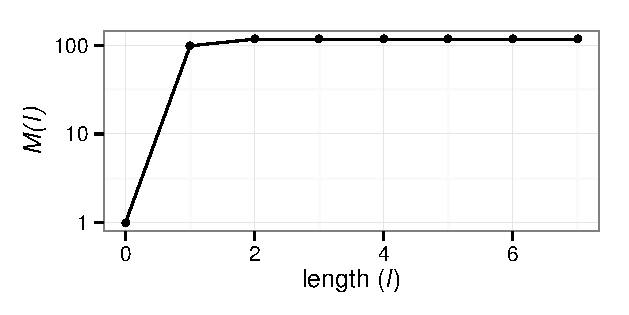
\includegraphics[width=0.75\textwidth]{length_plot.pdf}
	\caption{Average number of nodes $M(l)$ within a distance less than or equal to $l$ from any given vertex, for the 2012 agricultural commodity shipping network.}
	\label{fig:plot length}
\end{figure}


\begin{figure}[h]
	\centering
	\begin{subfigure}[b]{0.5\textwidth}
		\centering
        	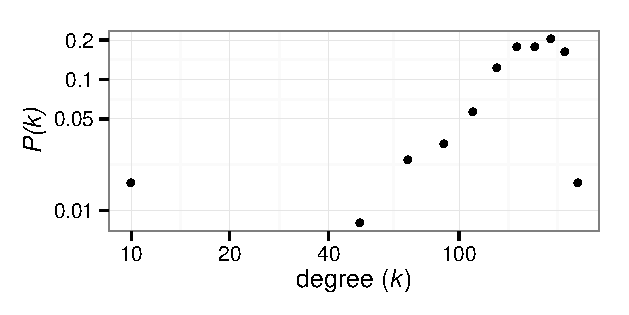
\includegraphics[width=\textwidth]{degree_dist.pdf}
        	\caption{Degree distribution $P(k)$}
        	\label{fig:degree dist}
	\end{subfigure}
	\hfill
	\begin{subfigure}[b]{0.5\textwidth}
		\centering
        	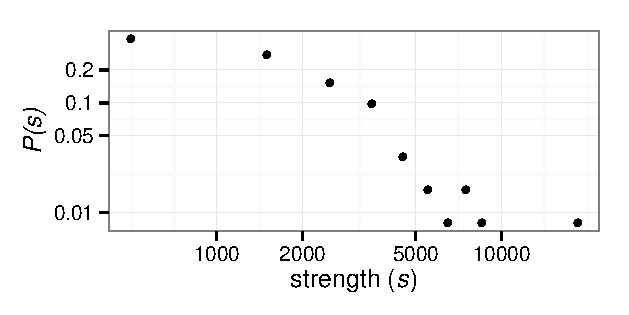
\includegraphics[width=\textwidth]{strength_dist.pdf}
        	\caption{Strength distribution $P(s)$}
        	\label{fig:strength dist}
	\end{subfigure}
	\hfill
	\begin{subfigure}[b]{0.5\textwidth}
		\centering
    		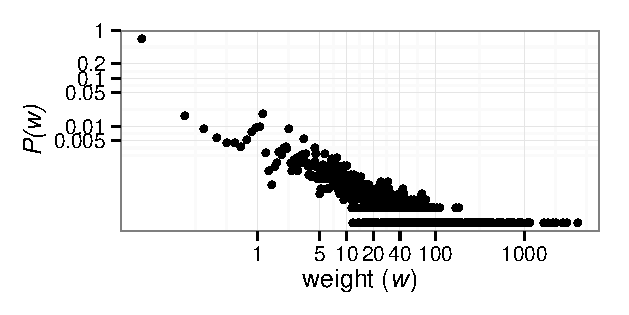
\includegraphics[width=\textwidth]{weight_dist.pdf}
   		\caption{Weight distribution $P(w)$}
        	\label{fig:weight dist}
	\end{subfigure}
	\caption{Network characteristic distributions for the 2012 agricultural commodity shipping network}
	\label{fig:distributions}
\end{figure}
		
		
				

\begin{figure}[h]
	\centering
		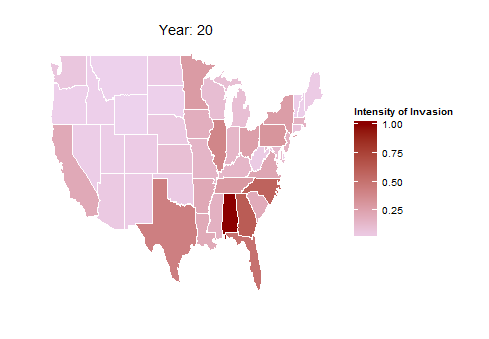
\includegraphics{agprod.png}
	\caption{Year 20 choropleth map of projected invasive fire ant spread from Alabama and transported via agricultural products. Growth rate of $r = 0.01$ was used. The plot shows the aggregate result from 100 simulations.}
	\label{fig:spread map}
\end{figure}

\begin{figure}[h]
	\begin{center}
		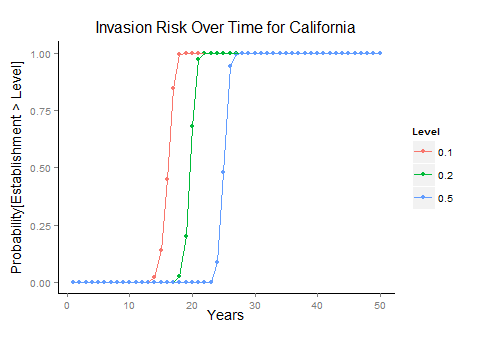
\includegraphics{riskcurve.png}
	\end{center}
	\caption{Risk curves for probability of passing establishment threshold in California. Plot shows aggregate result of 150 runs with 50 years in each. The simulations were initialized with Alabama fully established and growth rate $r = 0.01$ using data on agricultural products shipped by truck. }
	\label{fig:risk curve}
\end{figure}



\end{document}

















